%%%%% START PREAMBLE HEADER %%%%%

%%% START REQUIRED PACKAGES %%%

\documentclass[10pt]{report}
\usepackage{xcolor} 
\usepackage[a4paper, total={5.5in, 10in}]{geometry} 
\usepackage{lipsum}
\usepackage{hyperref}
\usepackage{graphicx}
\usepackage{babel}
\usepackage{setspace}
\usepackage{fontspec}
\usepackage{amsmath}
\setmainfont{Times New Roman}
\spacing{1.5}
\usepackage[superscript,biblabel]{cite}
\usepackage[export]{adjustbox}
\usepackage{amsmath}
\hypersetup{colorlinks=true,linkcolor=blue,filecolor=magenta,urlcolor=cyan,citecolor=blue}

%%% END REQUIRED PACKAGES %%%                


%%% START NEW COMMANDS new (shortcut) %%%

% This is a paragraph with normal font
\newcommand{\np}[1]{\paragraph{\normalfont{#1}}}
% This is a text with a color
\newcommand{\ct}[2]{\textcolor{#1}{#2}}
% This is a bold text 
\newcommand{\bt}[1]{\textbf{#1}}
% This is an italic text 
\newcommand{\et}[1]{\emph{#1}}
% This is an underline text 
\newcommand{\ut}[1]{\underline{#1}}
% This is a newline shortcut
\newcommand{\n}{\\}
% This is an equation shortcut
\newcommand{\ec}[1]{\begin{center} $#1$ \end{center}}
% Table title with bold text and correct space%
\newcommand{\dbar}{{d\mkern-7mu\mathchar'26\mkern-2mu}}

%%% END NEW COMMANDS (shortcuts) %%%


%%% START TITLE SETTINGS %%%
\title{\bt{Métodos experimentales para la determinación de la cmc, a partir de la determinación de la tensión superficial}}
\author{Pérez Alvarado Luis Raymundo, Facultad de Química, UNAM}
\date{04 de Enero de 2021}
%%% END TITLE SETTINGS %%%

%%%%% END PREAMBLE HEADER %%%%%
\begin{document}
    \maketitle


    \section*{Introducción}

    La tensión superficial esta relacionada con la fuerza y el trabajo, por lo que para su mejor entendimiento es necesario recordar sus definiciones.

    \subsection*{Teorema del trabajo \cite{web:trabajo} }

    El trabajo infinitesimal $dw$ se define como el producto de la fuerza $f$ por el desplazamiento $dx$.

    \ec{dw=Fdx=FdsCos\theta}

    En la ecuación anterior tenemos la forma diferencial del trabajo, en este caso se muestra de forma escalar para facilidad su trabajo.

    Se realiza la integración del trabajo a lo largo de la trayectoria de un punto a,b considerando que el ángulo es igual a cero.

    \ec{\int_{a}^b dw = F\int_{x_1}^{x_2} dx}

    \ec{w = F(x_2-x_1) = F\Delta x}

    \ec{w = F\Delta xCos\theta}

    Con las ecuaciones anteriores sabemos que podemos definir al trabajo como el producto de la fuerza por el desplazamiento y l componente del ángulo de la fuerza con respecto a la dirección del desplazamiento.

    \subsection*{Termodinámica de interfase \cite{web:tension} \cite{web:tensionValencia} \cite{web:tensionFQ} \cite{isotermaGibbs} \cite{web:Termo}}

    Consideramos la ecuación de la energía interna 

    \ec{du = dw + dq}

    En un sistema donde $dq=0$ la diferencial de energía interna es el diferencial del trabajo  

    \ec{du = dw = -pdv}

    En el caso de las superficies también hay una relación entre el trabajo y el área superficial, la cual es relacionada con el coeficiente $\gamma$ siendo 
    
    \ec{dw = -pdv+\gamma ds}

    En un sistema a presión y volumen constante tendremos que :

    \ec{du = dw = \gamma ds}

    El coeficiente $\gamma$ es conocido como la tensión superficial, la cual al ser despejada y puede expresarse verse de dos formas.

    \ec{\gamma = \frac{du}{ds} = \frac{dw}{ds}}

    Donde $\gamma$ puede ser interpretada como la cantidad de energía o trabajo necesaria para cambiar deformar una superficie.

    Con lo anterior se integra el diferencial del trabajo y de área.

    \ec{\int_{x}^y dw = \gamma \int_{s_1}^{s_2} ds} 

    \ec{w = \gamma \Delta S} 

    Con las relaciones planteadas se pueden entender mejor el fundamento de la tensión superficial, la cual es la base para poder expresarla en términos de propiedades medibles.

    \section*{Métodos de tensión superficial \cite{web:metodos12} \cite{web:metodosandes} \cite{web:metodosMadridi} \cite{web:metodosInge}}

    Se mostrarás el procedimiento experimental y las ecuaciones que usa cada método para determinar el valor de la tensión superficial.

    \subsection*{Método de la placa (Wilhelmy)}

    Este este método se usa una placa de vidrio o platino muy delgada la cual será sumergida por medio de un tensiómetro a una solución de la cual queremos calcular la tensión superficial.

    En este método se debe considerar se debe conocer perfectamente la geometría de la placa, ya que en base a esta se podrá determinar la tensión superficial.

    \begin{figure}[h]
        \centering
        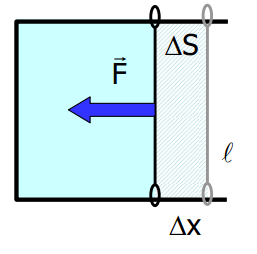
\includegraphics[scale=0.5]{./placa.png}
        \caption{Superficie desplazada.}
    \end{figure}

    En el esquema mostrado se puede apreciar la relación que existe entre la $\Delta x$ y $\Delta s$ teniendo la siguiente relación.

    \ec{\Delta S= l\Delta x}

    Como se considera que se esta trabajando con una placa, y esta tiene dos superficies esta se multiplica por 2 para considerar ambas ambas caras de la placa, resultando que $\Delta s$ para una placa es:

    \ec{\Delta S= 2l\Delta x}   

    Lo anterior es valido considerando que el ángulo $\theta$ con el cual esta placa es desplazada es igual a 0, siendo que $Cos(0)=1$, en caso de que no sea $\theta\neq 0 $ se deberá considerar el $Cos\theta$, además de considerar que $2l$ es una simplificación de $2(a+l)$ en el caso donde se cumple que el ancho es mucho menor que el largo de la placa $a<<l$.

    Usando la ecuación anterior y sustituyendo en la ecuación del trabajo para la tensión superficial tenemos lo siguiente.

    \ec{w = 2\gamma l\Delta x}

    Después, considerando la ecuación del trabajo, podemos relacionar a la fuerza por medio del trabajo.

    \ec{w = 2\gamma l\Delta x = F\Delta x}

    Al despejar la tensión superficial tenemos la expresión de la tensión superficial para una placa con ángulo $\theta=0$ y con ancho despreciable.

    \ec{\gamma = \frac{F}{2l}}

    De forma experimental parte de la placa entra en contacto con el líquido de forma vertical para que el ángulo $\theta=0$, por medio de un tensiómetro este es desplazado verticalmente para ser separado de la superficie del líquido y se calcula la fuerza que se requirió para ser separada, en el siguiente esquema se muestra el proceso realizado por el tensiómetro.

    \begin{figure}[h]
        \centering
        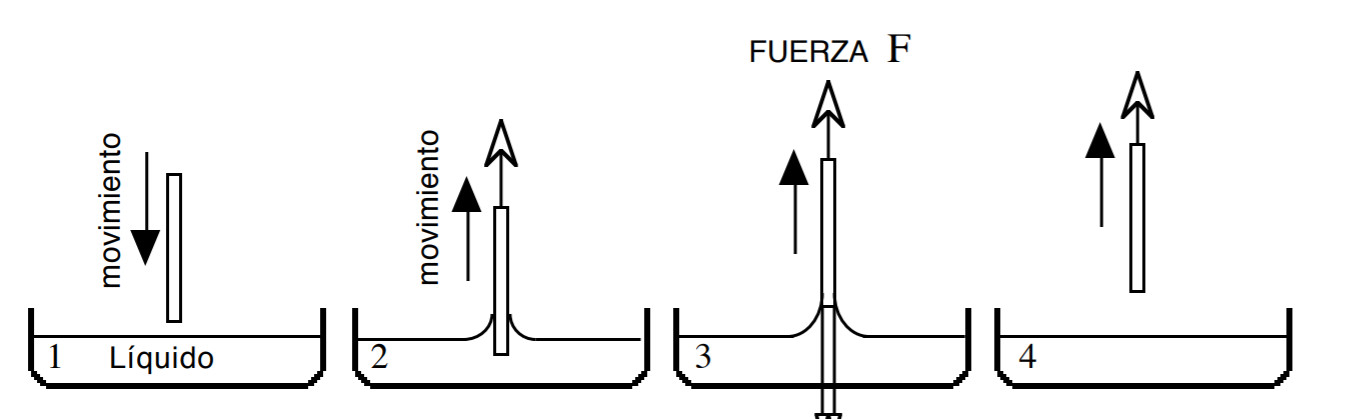
\includegraphics[scale=0.5]{./placaProcedimiento.jpg}
        \caption{Método de la placa.}
    \end{figure}

    En el esquema se puede ver que la placa tiene la contribución de dos fuerzas justo antes de poder ser separado de la superficie del líquido.

    El trabajo total realizado será la suma del trabajo de la placa más el trabajo de la fuerza de la tensión superficial.

    \ec{w_{total} = w_{placa}+w_{tensión}}

    La ecuación anterior muestra el balance de las fuerzas que intervienen en el sistema de estudio.
    
    Anteriormente se definió el trabajo de la tensión, sustituimos en la ecuación del trabajo total y se obtienen la siguiente ecuación.

    \ec{w_{total} = w_{placa}+2\gamma l}

    La expresión anterior se conoce como ecuación de Wilhelmy, con la cual es posible el determinar la tensión superficial.

    \ec{\gamma = \frac{w_{total}-w_{placa}}{2l}}

    En cual la diferencia de entre ambos trabajos será el trabajo que realiza el tensiómetro para poder separar la placa de la superficie.

    \ec{\gamma = \frac{F_{tensiómetro}}{2l}}

    Es decir que al realizar las mediciones con el tensiómetro obtenemos el trabajo realizado y al tener el perímetro de la placa se puede calcular la tensión superficial de una solución.

    \begin{figure}[h]
        \centering
        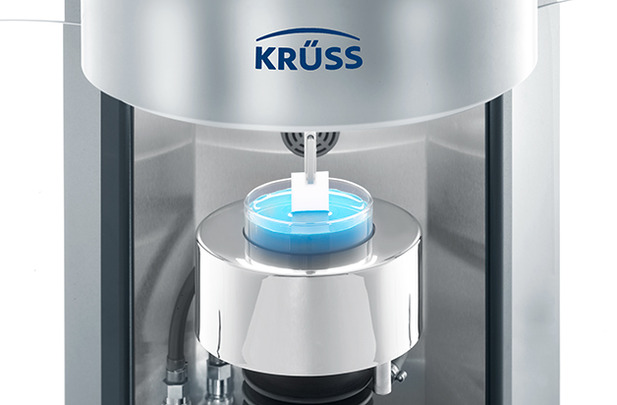
\includegraphics[scale=0.25]{./placaKrauss.jpg}
        \caption{Tensiómetro de marca Krauss.}
    \end{figure}

    Los tensiómetros actuales al conocer esta información son capaces de calcular la tensión superficial del liquido y recolectar una mayor cantidad de datos con mayor exactitud.


    \subsection*{Método del anill (Du Noüy)}

    Este método es muy similar en procedimiento experimental al de la placa con la diferencia de que ahora en lugar de estar en contacto una placa se usa un anillo de platino, el cual el sumergido en la superficie del liquido muy lentamente, de igual manera el ángulo es cero así que debe introducirse de forma vertical, se muestra un diagrama del proceso experimental.

    \begin{figure}[h]
        \centering
        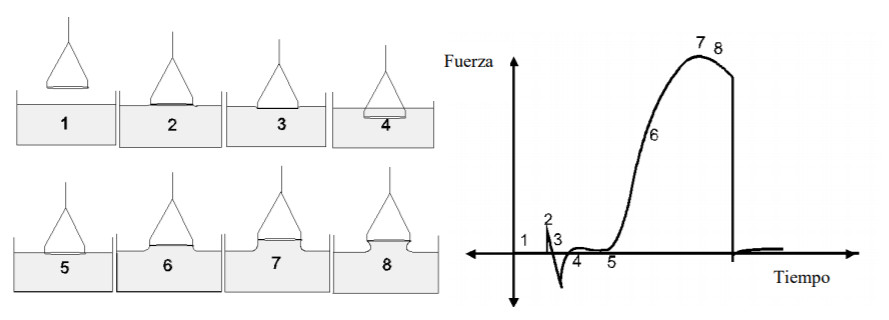
\includegraphics[scale=0.75]{./metodoAnillo.jpg}
        \caption{Tensiómetro de Du Noüy.}
    \end{figure}    

    Este método es muy similar al método de la placa ya que se basa en el mismo principio en donde para calcular la tensión superficial se usa el trabajo total en la cual es sistema tiene la misma forma, con la diferencia de que ahora se considera la geometría de la de un anillo, en el siguiente esquematiza la forma del anillo que se usa.

    \begin{figure}[h]
        \centering
        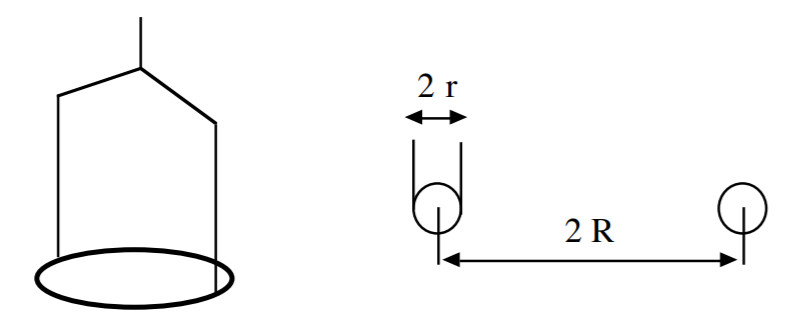
\includegraphics[scale=0.5]{./geometriaAnillo.jpg}
        \caption{Geometría del anillo.}
    \end{figure}

    Usando la ecuación de la tensión superficial de forma general tenemos la siguiente expresión: 

    \ec{\gamma = \frac{F_{tensiómetro}}{2p}}

    Donde $p$ es el perímetro de la geometría de la superficie que interacciona con la interfase del liquido, viendo el esquema podemos apreciar que es el perímetro de un circulo que es $p=2\pi r$, sustituimos el perímetro en la ecuación.

    \ec{\gamma = \frac{F_{tensiómetro}}{4\pi r}}

    La anterior es la ecuación con la que se determina la tensión superficial, pero esta misma se demostró que presenta un error asociado de hasta un 25\% esto debido al radio del anillo, por ello es necesario ingresar una constante para hacer una corrección en el calculo de la tensión superficial, la corrección es una función que depende del radio del anillo, la cual es dada por el fabricante del anillo, finalmente la expresión queda de la siguiente forma. 

    \ec{\gamma = \frac{kF_{tensiómetro}}{4\pi r}}

    El tensiómetro de análogo para su medición se le nombra al igual que el método Du Noüy. 

    \begin{figure}[h]
        \centering
        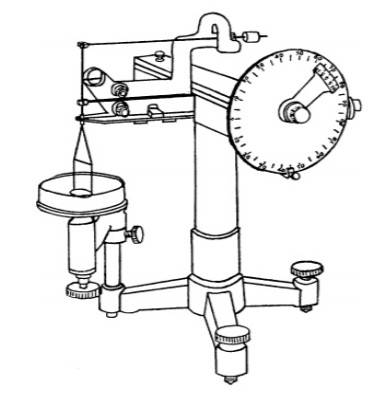
\includegraphics[scale=0.5]{./tensiometro.jpg}
        \caption{Tensiómetro de Du Noüy.}
    \end{figure}


    \subsection*{Método de volumen de gota}

    Este método consiste en el la formación de gotas del líquido de estudio en un capilar el cual esta en posición vertical, este método es análogo al método de pesada de gota.

    \begin{figure}[h]
        \centering
        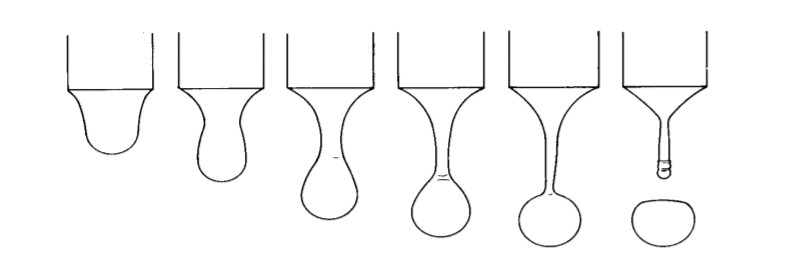
\includegraphics[scale=0.5]{./metodoPesada.jpg}
        \caption{Formación y caída de gotas.}
    \end{figure}

    Se retoma la ecuación del trabajo y la tensión superficial, la fuerza que esta presente cuando una gota en un capilar de forma vertical es el peso de la gota.

    \ec{w_{total} = 2\pi r = F = mg }

    Despejando la tensión obtenemos que la tensión esta en función de la masa dicha ecuación nos sirve para calcular la tensión cuando se pesa la masa de la gota.

    \ec{\gamma = \frac{mg}{2\pi rf}}

    La constante f es una constante que se calcula de forma experimental y depende del líquido usado.
    
    Por medio de la densidad del líquido, se sustituye la masa por el volumen de a gota por la densidad del líquido, quedando la siguiente expresión.

    \ec{\gamma = \frac{vd}{2\pi rf}}

    Con esta expresión podemos determinar la tensión superficial al conocer el volumen de una gota, la densidad del líquido y e factor de corrección para el líquido estudiado.

    \subsection*{Determinación del la concentración micelar crítica. \cite{art:arabian}}

    La concentración micelar crítica(CMC) es un intervalo en el cual empiezan a formarse los agregados supramoleculares, esta puede determinarse por medio de diversas propiedades, las cuales cambian de forma abrupta al llegar a dicha concentración.

    En la siguiente figura se muestran como se modifican algunas propiedades al llegar a la CMC.

    \begin{figure}[h]
        \centering
        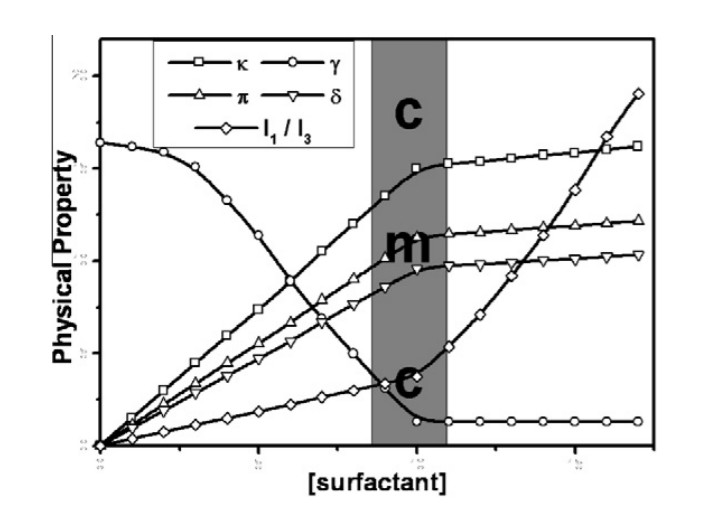
\includegraphics[scale=0.5]{./cmc.jpg}
        \caption{Cambio de propiedades al llegar a la CMC.}
    \end{figure}

    Por medio de la tensión superficial es posible determinar la CMC mediante métodos gráficos de tensión superficial vs concentración el logaritmo de su concentración, u otros como el usar la presión superficial y el logaritmo de la fracción molar que es mas preciso.

    \subsubsection*{Intersección de las rectas}

    En este método se grafica al tensión superficial contra el logaritmo de la concentración del anfifilo, pese a no ser tan exacto y puede variar el valor de la CMC ya el método es subjetivo ya que el experimentador decide los puntos que conforman la recta.

    Se mostraran gráficas donde se determino la CMC.

    \begin{figure}[h!]
        \centering
        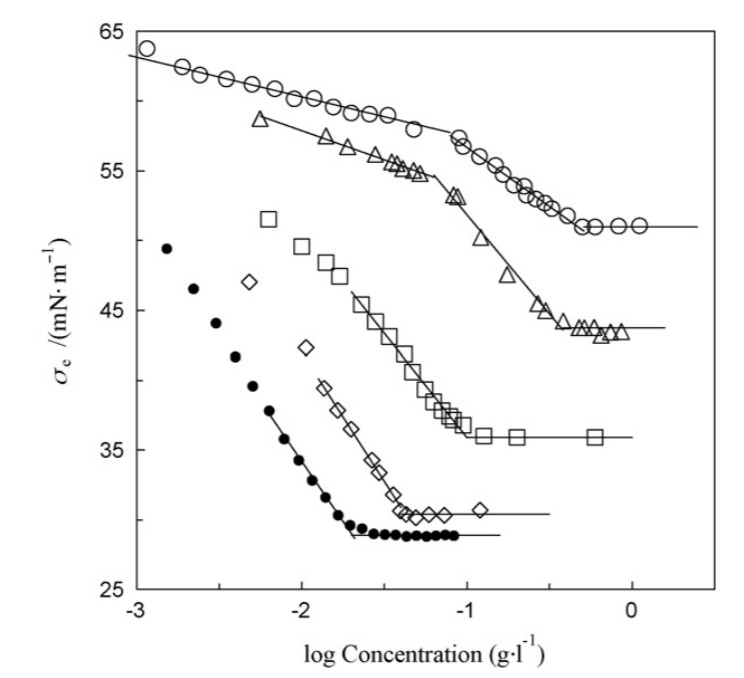
\includegraphics[scale=0.5]{./log1.jpg}
        \caption{Tensión superficial vs logaritmo de la concentración de etoxilatos de nonilfenol.\cite{art:log1}}
    \end{figure}

    \begin{figure}[h!]
        \centering
        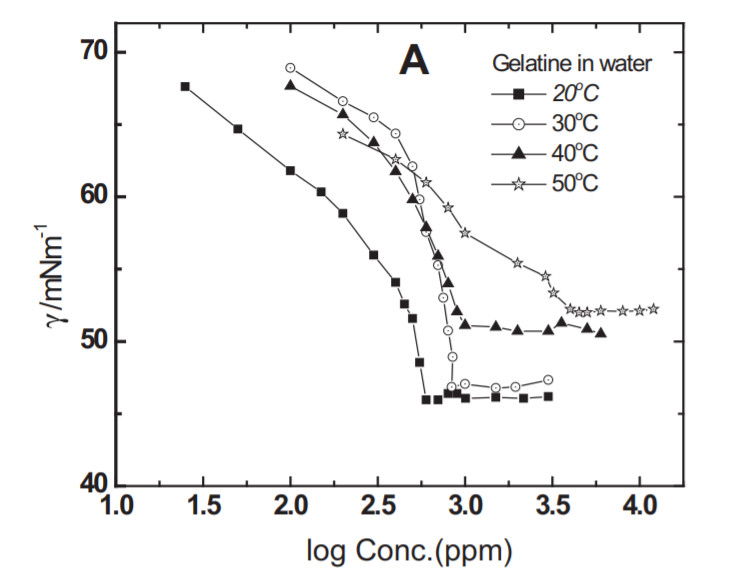
\includegraphics[scale=0.5]{./log2.jpg}
        \caption{Tensión superficial vs logaritmo de la concentración de gelatina.\cite{art:log2}}
    \end{figure}

    \subsubsection*{CMC con isoterma de Langmiur}

    En esta se grafica la presión superficial y el logaritmo natural de la fracción del surfactante, en la cual la presión superficial se vuelve constante cuando la fracción mol en donde inicia la CMC.

    \begin{figure}[h!]
        \centering
        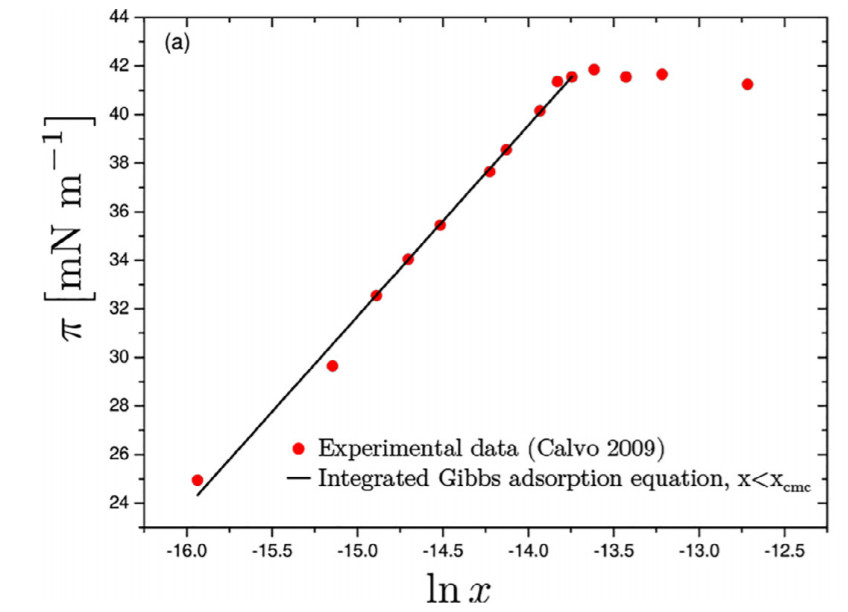
\includegraphics[scale=0.5]{./iso1.jpg}
        \caption{Presión superficial vs logaritmo natural de la fracción mol del etoxilato de nonilfenol.\cite{art:iso1}}
    \end{figure}

    \begin{figure}[h!]
        \centering
        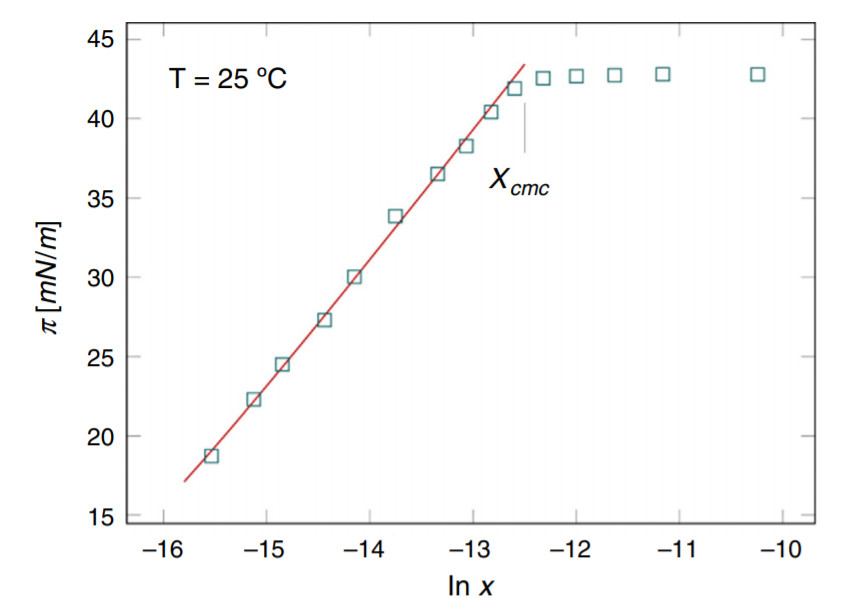
\includegraphics[scale=0.5]{./iso2.jpg}
        \caption{Presión superficial vs logaritmo natural de la fracción mol del pt-Octilfenol.\cite{art:iso2}}
    \end{figure}

    Por medio de la ecuación de la isoterma de Langmiur se puede calcular la fracción mol de saturación la cual es la fracción molar de la CMC es un método mucho más precioso para determinar la CMC.

    \begin{figure}[h!]
        \centering
        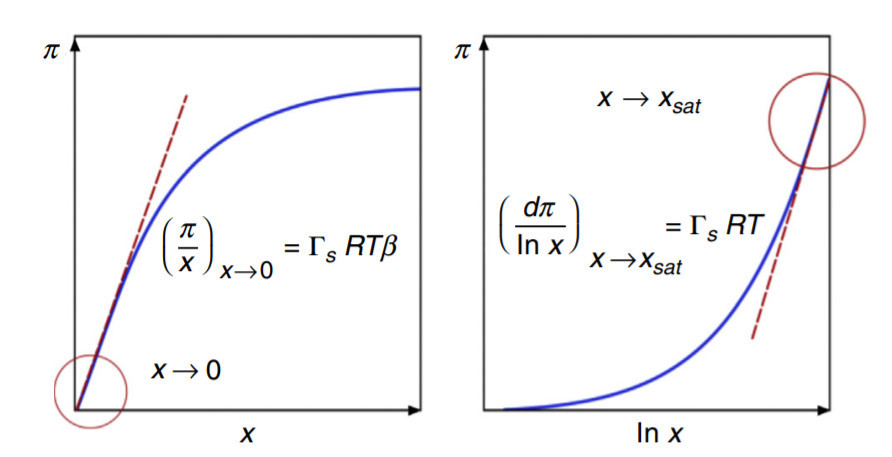
\includegraphics[scale=0.75]{./isoLag.jpg}
        \caption{Curva teórica de la isoterma de Langmiur.\cite{art:iso2}}
    \end{figure}




    %% START REFERENCES %% 

    % DEFINE STYLE FORMAT%
    \bibliographystyle{ieeetr}
    % SPECIFY THE FILE NAMEw %
    \bibliography{references}

    %% END REFERENCES %% 


\end{document}